\documentclass[tikz,crop]{standalone}
\usepackage{amsmath}
\usetikzlibrary{positioning}
\usetikzlibrary{calc}
\usetikzlibrary{arrows.meta}
\pagestyle{empty}

\tikzset{
  arr/.style={{Circle[length=3pt]}->,shorten <=-1.5pt}
}

\begin{document}
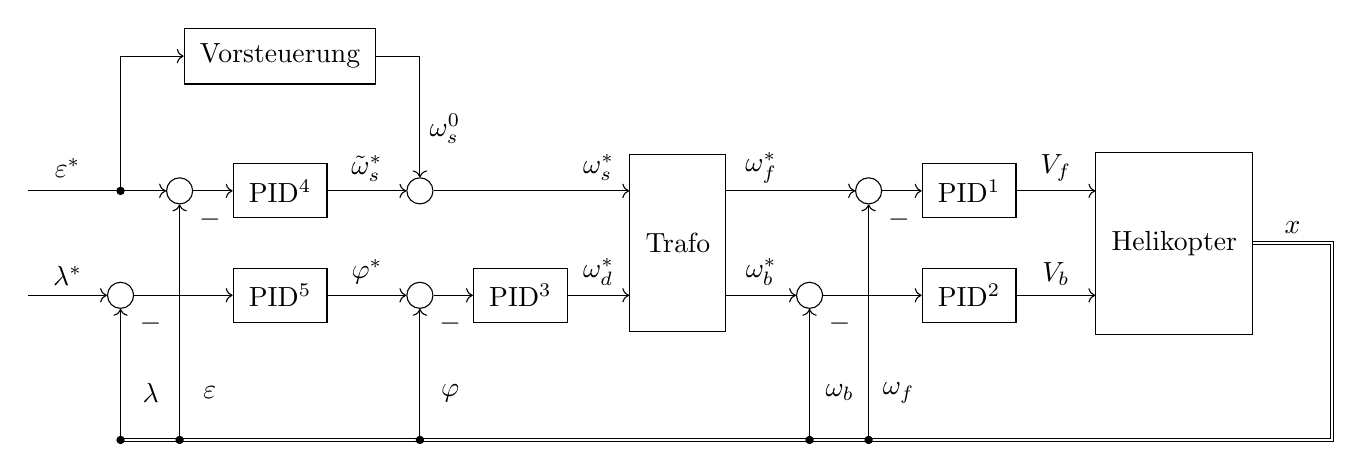
\begin{tikzpicture}
    %\draw [help lines] (-20, -5) grid (5, 5);
    \node [draw, inner ysep=1 cm, inner xsep = 0.2 cm] (heli) at (0, 0) {Helikopter};
    \coordinate [above left = -0.5cm and 0cm of heli] (heli_f);
    \coordinate [below left = -0.5cm and 0cm of heli] (heli_b);
    \coordinate [left = 0cm of heli] (heli_w);
    \node [left = of heli_f, draw,inner sep = 0.2 cm] (pd_wf) {PID\textsuperscript{1}};
    \node [left = of heli_b, draw,inner sep = 0.2 cm] (pd_wb) {PID\textsuperscript{2}};
    \node [draw, shape=circle, left=0.5cm of pd_wf] (sum_wf) {};
    \node [draw, shape=circle, left=1.25cm of pd_wb] (sum_wb) {};
    \coordinate [left = 1.5cm of sum_wb] (trafo_x);
    \node at (trafo_x |- heli) [draw, inner ysep = 1 cm, inner xsep = 0.2 cm] (trafo) {Trafo};
    \coordinate [right=0cm of trafo] (trafo_e);
    \coordinate [left=0cm of trafo] (trafo_w);
    \node at ({$(trafo) + (-2,0)$} |- heli_b) [draw,inner sep = 0.2 cm] (phi_pid) {PID\textsuperscript{3}};
    \node [left = 0.5 cm of phi_pid,draw,shape=circle] (sum_phi) {};
    \node at (sum_phi |- heli_f) [draw,shape=circle] (sum_ws) {};
    \node [left=of sum_ws,draw,inner sep = 0.2 cm] (eps_pid) {PID\textsuperscript{4}};
    \node at (eps_pid |- sum_phi) [draw,inner sep = 0.2 cm] (lamb_pid) {PID\textsuperscript{5}};
    \node [above = of eps_pid,draw,inner sep = 0.2 cm,xshift=0cm] (vs) {Vorsteuerung};
    \node [left = 0.5 cm of eps_pid,draw,shape=circle] (sum_eps) {};
    \node [left = 1.25cm of lamb_pid,draw,shape=circle] (sum_lamb) {};
    \coordinate [left = of sum_lamb] (start_lamb);
    \coordinate (start_eps) at (start_lamb |- sum_eps);

    \node [below right=0cm of sum_wf] (wf_minus) {$-$};
    \node [below right=0cm of sum_wb] (wb_minus) {$-$};
    \node [below right=0cm of sum_phi] (phi_minus) {$-$};
    \node [below right=0cm of sum_eps] (eps_minus) {$-$};
    \node [below right=0cm of sum_lamb] (lamb_minus) {$-$};


    \draw [->] (pd_wf) -- (heli_f) node (Vf_label) [midway,above] {$V_f$};
    \draw [->] (pd_wb) -- (heli_b) node [midway,above] {$V_b$};
    \draw [->] (sum_wf) -- (pd_wf);
    \draw [->] (sum_wb) -- (pd_wb);
    \draw [->] (trafo_e |- sum_wb) -- (sum_wb) node (wb_label) [midway,above] {$\omega_b^*$};
    \draw [->] (trafo_e |- sum_wf) -- (sum_wf) node at (Vf_label -| wb_label) (wf_label) {$\omega_f^*$};
    \draw [->] (phi_pid) -- (phi_pid -| trafo_w) node (wd_label) [midway,above] {$\omega_d^*$};
    \draw [->] (sum_phi) -- (phi_pid);
    \draw [->] (sum_lamb) -- (lamb_pid);
    \draw [->] (sum_ws) -- (sum_ws -| trafo_w) node at (wf_label -| wd_label) (ws_label) {$\omega_s^*$};
    \draw [->] (eps_pid) -- (sum_ws) node [midway,above] (delta_ws_label) {$\tilde{\omega}_s^*$};
    \draw [->] (lamb_pid) -- (sum_phi) node at (delta_ws_label |- wd_label) {$\varphi^*$};
    \draw [->] (sum_eps) -- (eps_pid);
    \draw [->] (vs) -| (sum_ws) node [right,pos=0.8] {$\omega_s^0$};
    \draw [->] (start_lamb) -- (sum_lamb) node [midway,above] (lamb_label) {$\lambda^*$};
    \draw [->] (start_eps) -- (sum_eps) node at (lamb_label |- ws_label) {$\varepsilon^*$};

    \draw [double] (heli) -- ++(2,0) node [midway,above] {$x$} -- ++(0, -2.5) coordinate (base) -- (sum_lamb |- base);

    \draw [arr] (sum_eps -| sum_lamb) |- (vs);

    \draw [arr] (base -| sum_wf) -- (sum_wf) coordinate [pos=0.2] (feedback_label) node at (feedback_label -| wf_minus) {$\omega_f$};
    \draw [arr] (base -| sum_wb) -- (sum_wb) node at (feedback_label -| wb_minus) {$\omega_b$};
    \draw [arr] (base -| sum_phi) -- (sum_phi) node at (feedback_label -| phi_minus) {$\varphi$};
    \draw [arr] (base -| sum_eps) -- (sum_eps) node at (feedback_label -| eps_minus) {$\varepsilon$};
    \draw [arr] (base -| sum_lamb) -- (sum_lamb) node at (feedback_label -| lamb_minus) {$\lambda$};

\end{tikzpicture}
\end{document}